% Sample LaTeX file for creating a paper in the Morgan Kaufmannn two
% column, 8 1/2 by 11 inch proceedings format.

\documentclass[letterpaper]{article}
\usepackage{proceed2e, amsmath, graphicx}
\usepackage[margin=1in]{geometry}

% Set the typeface to Times Roman
\usepackage{times}

\title{Distributed Deep Neural Training with ADMM}

\author{} % LEAVE BLANK FOR ORIGINAL SUBMISSION.
          % UAI  reviewing is double-blind.

% The author names and affiliations should appear only in the accepted paper.
%
%\author{ {\bf Harry Q.~Bovik\thanks{Footnote for author to give an
%alternate address.}} \\
%Computer Science Dept. \\
%Cranberry University\\
%Pittsburgh, PA 15213 \\
%\And
%{\bf Coauthor}  \\
%Affiliation          \\
%Address \\
%\And
%{\bf Coauthor}   \\
%Affiliation \\
%Address    \\
%(if needed)\\
%}

\begin{document}

\maketitle

\begin{abstract}
The project investigates the ways of breaking down deep neural network processing between several computational units. Some existing approaches to the problem are summarized based on a relevant literature review.
An algorithm utilising the Alternating Direction Method of Multipliers (ADMM) optimization within Deep Learning is proposed. It is then thoroughly tested and refactored, considering the technical limitations of the deep learning framework used - Caffe. Finally, the complete and working version of the algorithm is obtained.
The classification accuracy achieved by the dual setup on CIFAR10 is found to be within 6\% and on MNIST 0.5\% lower than the one achieved by a singular architecture. It is proven, however, that the novel setup is also able to accomodate a much larger batch size (factor of 2) which can be interpreted as a success and a major disruption. Prospectively, it allows for training of much deeper network topologies in an architecture distributed between several computational units.
\end{abstract}

\section{INTRODUCTION}

Understanding data was universally humanity's greatest feat and the need for it is even more compelling nowadays, when the size of datasets is becoming unimaginable. We want to classify more, do it faster and with ever less supervision from the user.

Novel machine learning methods have made great advancements in inference and classification tasks, but the hunger for more robust algorithms and setups grows even quicker. The scientific community has seen the rise and fall of popularity of neural networks in the 80s and 90s. A period of stagnation has followed, accompanied by an aggressive increase in the available computational power and resurrection of the neural nets in the form of deep learning. More power also means more complicated models, and hence the ability to represent complex functions. The additional processing layers in the deep networks are proven to be able to represent exponentially more complicated functions. An ideal piece of hardware suiting the needs of deep learning is a GPU, whose thousands of cores enable highly parallelized computation. As we near the technical limits of single computational units though, we have to turn our research efforts to using distributed approaches allowing us to harness an even increasing number of clock cycles. This paper presents a novel approach to distributing the computation developed by using a convex optimization algorithm known as ADMM, Alternating Direction Method of Multipliers. The method significantly cuts down the communication cost characteristic of the existing distributed approaches and at the same time offers an algorithmic guarantee of convergence.

This paper first introduces some background information about the deep neural networks and their relation to ADMM, summarizes some of the existing work on the distributed neural training and then goes on to explain the architectural and practical intricacies of the setup. It then goes on to present the important results confirming the validity of the initial problem statement and usefulness of the approach in general.
\section{BACKGROUND}

\subsection{MACHINE INTELLIGENCE}

A myriad of the datasets observed nowadays are non-linear - it's impossible to learn the underlying classification function by means of a simple logistic regression, linear in its parameters. Neural networks comprise of layers of interconnected logistic units which together form a lattice capable of representing highly complex non-linearities. The interdependencies between the units, the "neurons", are described by the weights of the edges between them. Deep networks consist of a number of those neural layers, with each one exponentially increasing the capability of the setup to learn complex functions. In convolutional networks, the weights between the neurons are in fact convolutional filters applied to the preceding layer's outputs. They build up hierarchical features of the input automatically, hence removing the need for hand-designing them. 

The networks automatically learn the parameters of convolutional filters that should be applied to the raw input images in order to obtain the desired label. As with traditional neural networks, the weights are learned by computing their gradient with respect to the overall classification error, defined as the 2-norm of the predicted and expected image labels. Two complimentary algorithms -  \textbf{forward} and \textbf{backward} \textbf{propagation} are executed during each iteration of training. The first one computes the activations of each of the neurons, while the second updates the parameters based on the calculated gradients.

\subsection{ADMM}

Alternating Direction Method of Multipliers is an algorithm for solving constrained optimisation problems. It is based on the augmented Lagrangian method, although uses partial updates to achieve the function objective. \\
The standard Lagrangian method aims to minimise a function f(x) subject to a set of constraints in the form gi(x) = 0. We do this by introducing another function L(x) which is a combination of the objective and the constraints like: $\min_{x} L(x) = f(x) + \boldsymbol{\lambda^T g(x)}$, where $\lambda$ is the vector of Lagrange multipliers.

In ADMM, we are trying to minimize a function of the form: $\min_{x} L(x) = f(x) + g(x)$ and to do that we introduce an auxiliary variable $y$, which will help us break the problem down into pieces that are easier to handle. $x$ and $y$ are dual variables and we will be attempting to minimise the difference between them. We are now facing a constrained optimisation problem of the form:
\begin{align}
\min_{x,y} L(x,y) = f(x) + g(y) \\
\textrm{subject to } x = y \Leftrightarrow x-y=0
\end{align}

which we can solve using Lagrange multipliers method as:
\begin{equation}
\label{ADMM_equation}
\min_{x,y} \max_{\lambda} L(x,y) + \lambda^T (x-y) + \beta ||x-y||^2
\end{equation}

where the last term is a regularisation minimising the difference between the dual variables.\\
The algorithm sequentially updates the x and y variables in order to achieve two objectives:
\begin{enumerate}
	\item Minimize the difference between them
	\item Minimize the overall loss
\end{enumerate}

\section{Previous work}

The two most notable works devoted to the field of distributed neural network training are those by Dean et al [1] and Chilimbi et al [2]. \\
The first work proposes a framework called DistBelief which parallelizes the training within and between the machines. It enables model parallelism through distributing the responsibility for different nodes' parameter computation between different machines. The parameters are stored centrally, though, on a dedicated parameter server. Due to the inherently sequential nature of Stochastic Gradient Descent two new alternatives are also introduced - Downpour SGD and Sandblaster L-BFGS. Both offer a parallel optimization through asynchronous updates of the network parameters and distributing their storage. Even though asynchronous, the method yields surprisingly stable and well performing results.\\
The second paper presents a similar approach, named Project Adam, where the parameter and computation servers are disjoint, but where the parameter updates are carried in an asynchronous, lock-free fashion. The model is partitioned vertically, with the convolutional layers separate from the fully connected ones. The forward and back propagations are executed on concurrent threads serving different images. Interestingly, even though this introduces races and usage of not-updated parameter values the overall setup does converge which nicely demonstrates neural nets' resilience to such noise. The approach extends to even 120 machines and trains the networks to an unprecedented accuracy on the MNIST dataset. \\

Both papers introduce approaches to distributing the deep network computation wildly different to the one presented in the following report. To cut down on the communication cost and still have an algorithmic guarantee of convergence, we turn to a convex optimization method called ADMM and apply it to out problem.


\section{ADMM and Deep Learning}

The idea of sequential dual parameter updates nicely extends to distributed neural setups. We can start with breaking down our deep neural network into two parts, duplicating one of the convolutional layers so as to be included in both of the resulting networks. The dual variables x and y will then correspond to the activations of the duplicated layers. The overall optimization is then going to entail two steps, analogous to the ones mentioned before: 1) minimizing the difference between the layer activations, 2) minimizing the difference between the predicted and actual image labels. Looking back at the underlying ADMM equation \ref{ADMM_equation}, the first step corresponds to minimizing $\beta||x-y||^2$, while the second one minimizes $L(x,y)$. This is neatly represented in figure \ref{broken}. We are using a single convolutional layer, in this case layer conv3, to serve as a breaking point and be included in both of the resulting nets through its dual counterparts.

\begin{figure}[h]
	{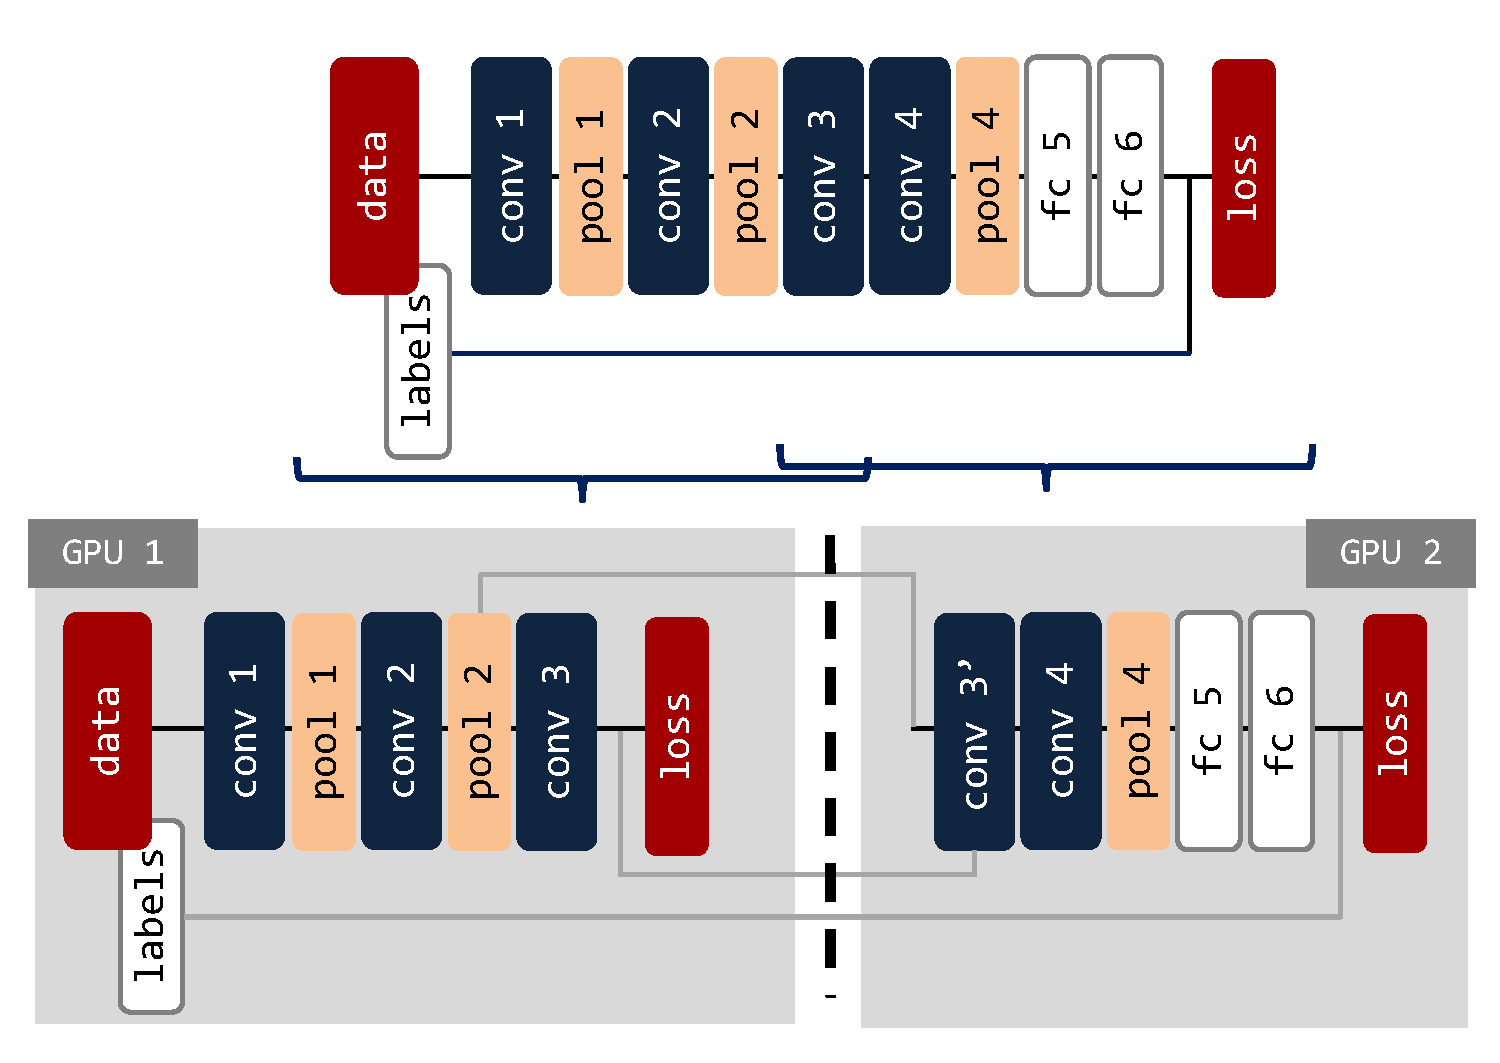
\includegraphics[width=3.15in]{broken}}
	\caption{Breaking down a deep neural topology to conform with the ADMM Algorithm.}
	\label{broken}
\end{figure}

The two separate networks now coexist and communicate through the shared layer activations. They are, however, inherently disjoint which is pronounced by the ability to train them on two separate processing units.

\section{Experimental setup}

The setup was implemented and tested using Caffe deep learning framework. The network parameters were stored on the same server, but managed separately and automatically by Caffe. The communication between the two networks was kept to minimum. 
The parameters that were mutually necessary for computation were:
\begin{enumerate}
	\item For \textbf{net1} - the output of conv3' layer in order to calculate the norm between the dual layers.
	\item For \textbf{net2} - the output of pool3 layer in order to make the input to both of the dual layers identical.
\end{enumerate}

Hence the communication overhead was limited to the activations of a convolutional and a pooling layer. This hold regardless of the size of the individual networks, and can be thus deemed to be significantly less expensive than parameter sharing in other distributed setups.

Based on the above considerations the algorithm was finalized as:
\begin{figure}[h]
	{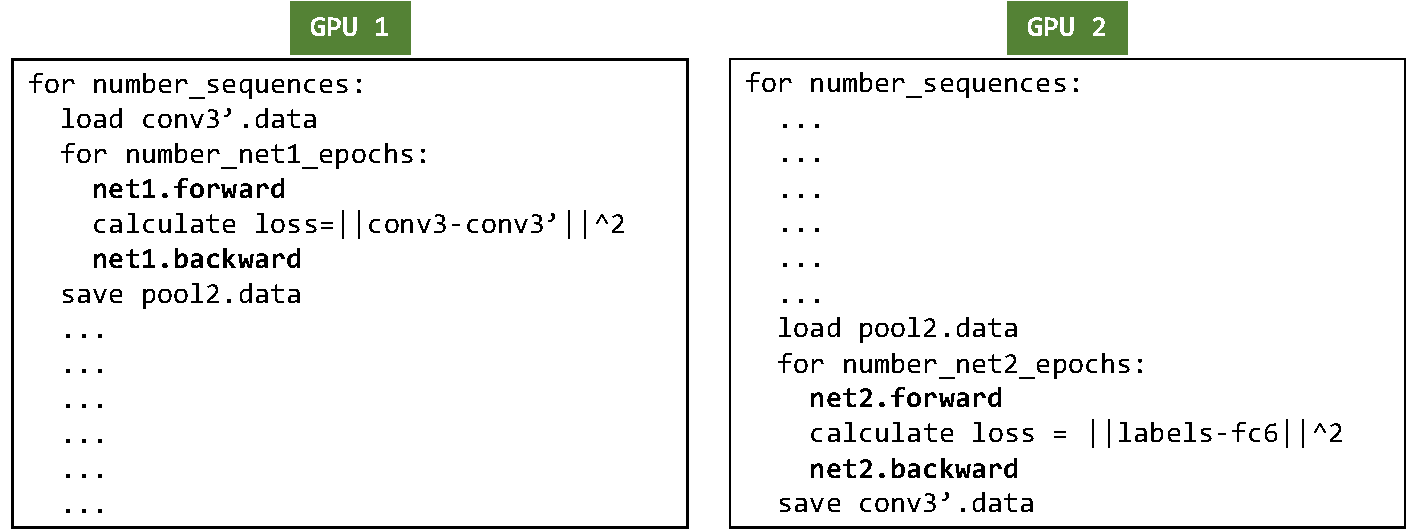
\includegraphics[width=3.15in]{algocode_revisited}}
\end{figure}

The networks' objectives are optimized separately and sequentially. Each one is trained for a predetermined number of epochs, while the other one is in an idle state, with its parameters staying constant.

The meta-parameters of the network were adjusted empirically. In order to provide a sound baseline, the parameters were chosen so that the networks were individually achieving the best observed performance. In order to reduce the user involvement in choosing the appropriate parameters in the future it is suggested that Bayesian Optimisation techniques are used.

In all cases the networks were trained until and subsequently compared against each other after convergence of the loss function was observed. This proved to be around 120 epochs for each of the tested setups.

The hardware used for training of the networks was an Nvidia GeForce GTX Titan graphical processing unit for each dual network, hence two of them in total.

\section{Performance metrics}

To validate the completion of the performance objectives, the newly designed dual architecture was contrasted with the corresponding traditional one from which it was sourced. The performance is defined based on the following metrics:
\begin{enumerate}
	\item Classification accuracy
	\item Convergence performance
	\item Training time
	\item Memory efficiency
\end{enumerate}

The last one should be considered the most crucial, since it is most closely related to the objective of the project, and hence can be used as a definite measure of its ultimate success. It can be indirectly measured by checking the maximum batch size that can be reasonably utilized for the training. The intuition behind that is simple - if the setup can accomodate for more data, it will as easily accomodate for a bigger model. 

\section{Results}

The dual and traditional setups presented above were tested on two distinct datasets, cifar10 and MNIST, widely known in the machine learning community. The following summary gives an overview of the performance achieved over both of the datasets over the metrics defined in the previous section.

\begin{figure}[h]
	\centerline{\includegraphics[width=3.15in]{final_2.png}}
	\caption{The final loss convergence pattern for the single and dual network architectures on cifar10 dataset. The step pattern for the training of the dual network is clear and visible, although the convergence trend is very pronounced and dominating over the idling periods.}
	\label{final_2}
\end{figure}

\begin{figure}[h]
	\centerline{\includegraphics[width=3.15in]{final_2.png}}
	\caption{The final loss convergence pattern for the single and dual network architectures on cifar10 dataset. The step pattern is now removed and only the non-idling iterations’ losses are shown.}
	\label{final_3}
\end{figure}

\begin{enumerate}
	\item The classification accuracy achieved after convergence of the networks was within a 6\% bound from the traditional setup in case of cifar10 dataset over three distinct trials. In MNIST, the accuracy was bound by 0.5\%. The exact results are presented in table \ref{results}. Within the deep learning community, where tenths of percent of classification accuracy improvement result from months of research, such a deficiency would be quite pronounced. This project’s main objective, though, was to increase the amount of data that can be used for training of a deep network while, at the same time, showing that such a network could successfully converge and classify. As such, the objective was most definitely met, and the $\mathtt{\sim}$5\% classification accuracy difference should be treated as a sign of successful training rather than performance deficiency. Further, it is a metric that most certainly has a potential for being improved.
	
	\begin{table}[h]
		\caption{The experimental classification accuracy results}
		\label{results}
		\begin{center}
			\begin{tabular}{lll}
				\multicolumn{1}{c}{\bf Dataset}  &\multicolumn{1}{c}{\bf Traditional accuracy} &\multicolumn{1}{c}{\bf Dual accuracy} \\
				\hline \\
				cifar10         &77.78\% &72.15\% \\
				MNIST             &99.14\% &98.73\%\\

			\end{tabular}
		\end{center}
	\end{table}
	
	\item The simplest way to analyse the convergence performance is looking at the training curves, particularly the ones presented in figures \ref{final_2} and \ref{final_3}. The first one clearly exhibits the expected step pattern due to the algorithm optimizing the networks sequentially one after another. It also contrasts it with the full training curve with the one for a single network. The convergence trend is evidently pronounced. The second figure pronounces the trend even more, contrasting the final training curves with the steps removed, and hence showing only the non-idle iterations. In all of the figures, the first one, net1 corresponds to the performance of the left part of the dual net, net2 to the right one, whereas net12 is the source architecture broken down in order to obtain the other 2.
	
	\item The training time is the total training time spent on convergence. This means that in case of the dual network it is calculated separately for network 1 and network 2, as only the latter should be contrasted with the value for a single network.\\
	It took 4 hours 21 minutes to train single network, on average. This is to be contrasted with 15 hours 54 minutes to train the dual one, with 1 hours 28 minutes spent on optimizing net 1's objective, and 14 hours 26 minutes spent on optimizing net 2's objective. It clearly takes a lot longer to train the dual network architecture, by a factor of 3.65.\\
	This can most definitely be considered a long time. Speeding up the training procedure was not, however, an objective of the project. Training two separate networks in a sequential manner involves  many operations more costly and less optimised as is the case in a well-developed framework like Caffe. Such a result should not constitute a reason to worry, though, as the main objectives of the project were met, whereas with further development the programmatic framework can be optimised for speed.
	
	\item The novel dual net architecture was predicted to be able to accommodate a batch size much bigger than the one in the traditional, singular network setup. During testing, the batch was increased to twice its previous size every time until it filled up the memory of the GPU completely. It turned out that:
	\begin{itemize}
		\item The biggest batch size that can be fitted on the single net topology is 2608 samples.
		\item The biggest batch size that can be fitted on the dual net topology is 4095 samples.
	\end{itemize}
	
	These results are outstanding - by breaking down the network between two units, we were able to increase the amount of data that can be processed on them together by a factor of two. This is undoubtedly one of the biggest successes of the project and a completion of the main objective - extending the size of data batches that can be used during deep network training.
\end{enumerate}

\section{Conclusions}

Let's recap on the initial objective of the project:

\textbf{"To design and implement an algorithm training a deep neural network on two separate machines, using the Alternating Direction Method of Multipliers technique to allow for the convergence of two network performance objectives"}

The two network performance objectives which we are trying to minimize are:
\begin{enumerate}
	\item For network 1 - the difference between the dual convolutional layers' values
	\item For network 2 - the difference between the computed image labels and the ground truth
\end{enumerate}

As proven in the previous section, both of those were duly met, since the losses for both networks converged and were thus optimised. This was additionally confirmed by comparing the performance of the dual network to the traditional unified approach. The performance, as measured by the classification accuracy, didn't differ by more than 6\% for cifar10, and an outstanding 0.5\% for MNIST.

The network architecture used was a heuristic choice. It bases itself quite heavily on the CaffeNet architecture, boasting popularity in the deep learning community. The 4 convolutional layers were broken down in two parts with conv1, conv2 and conv3 belonging to the first network and conv3p (the conv3 dual layer) and conv4 belonging to the second network.

Before the training started many problems were encountered with the sole setup of the framework. It turned out that a few critical components are not very well documented and hence the documentation had to be replaced with long hours of research and reading through the source code of the framework. Several technical compromises had to be made in order to bypass the unresolved bugs in the software. The most notable is the inability to initialise the dual conv3p as a MemoryData layer, which required its initialisation from a "dummy" LMDB file.

The classification results obtained were, while not perfect, promising, and most definitely point towards the success of the approach. It takes nearly 4 times longer to train the dual network setup, however speed of training was not one of the objectives and as such, shouldn't be taken as a fault of the framework.

Most successfully, though, the maximum batch size which could be fitted on the network architecture increased nearly by a factor of 2, which is the single most important and disrupting result of the project. It proves that the setup is much more memory efficient and hence allows for training much deeper, more complex neural topologies.

The future work will focus on breaking down the traditional architecture further in order to distribute the computation across many more servers.


\newpage

\subsubsection*{References}

J.~Dean, G.~Corrado, R.~Monga, K.~Chen, M.~Devin, M.~Mao, A.~Senior, P.~Tucker,
K.~Yang, Q.~V. Le, et~al.
\newblock Large scale distributed deep networks.
\newblock In {\em Advances in neural information processing systems}, pages
1223--1231, 2012.

T.~Chilimbi, Y.~Suzue, J.~Apacible, and K.~Kalyanaraman.
\newblock Project adam: Building an efficient and scalable deep learning
training system.
\newblock In {\em 11th USENIX Symposium on Operating Systems Design and
	Implementation (OSDI 14)}, pages 571--582, 2014.

\end{document}
